\begin{marginfigure}
	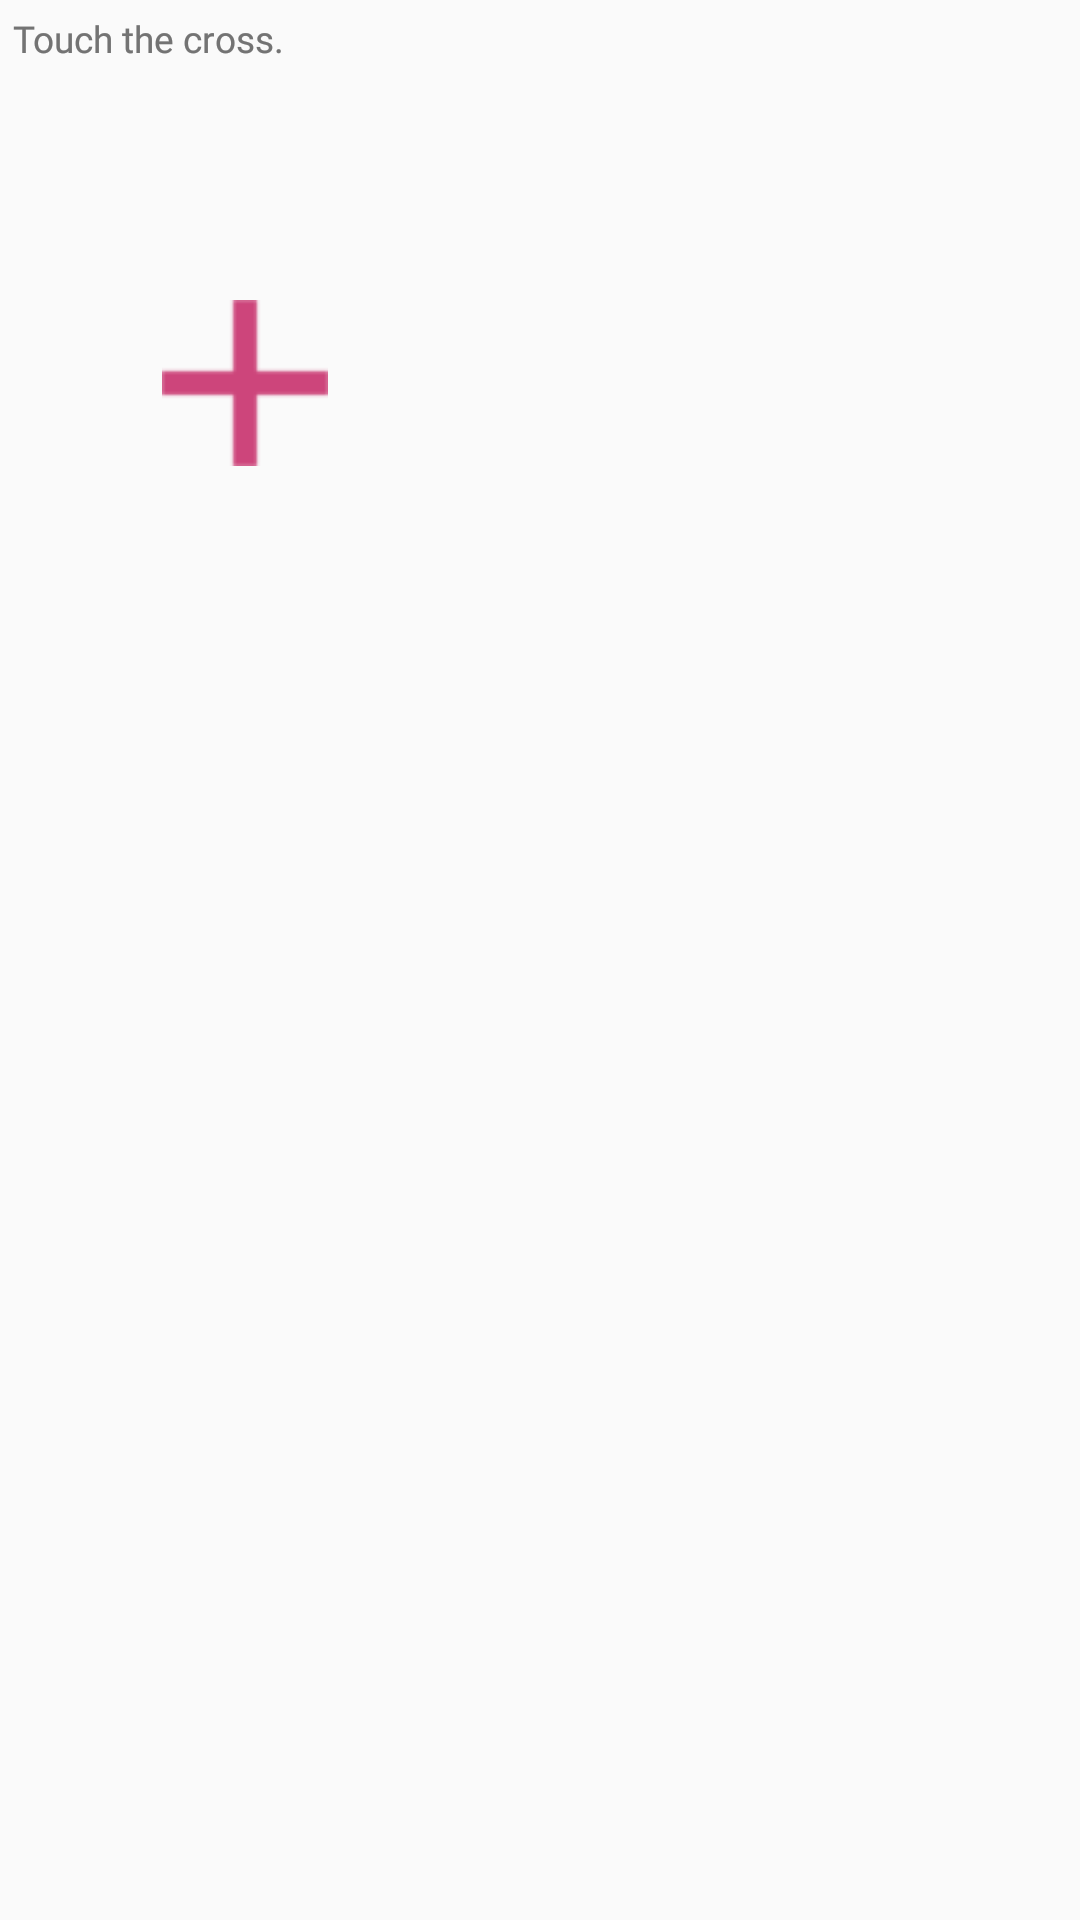
\includegraphics[height=\linewidth]{cross}
	\caption{Touch task with one cross displayed.\newline}
	\label{fig:touchtask}
\end{marginfigure}

\begin{marginfigure}
	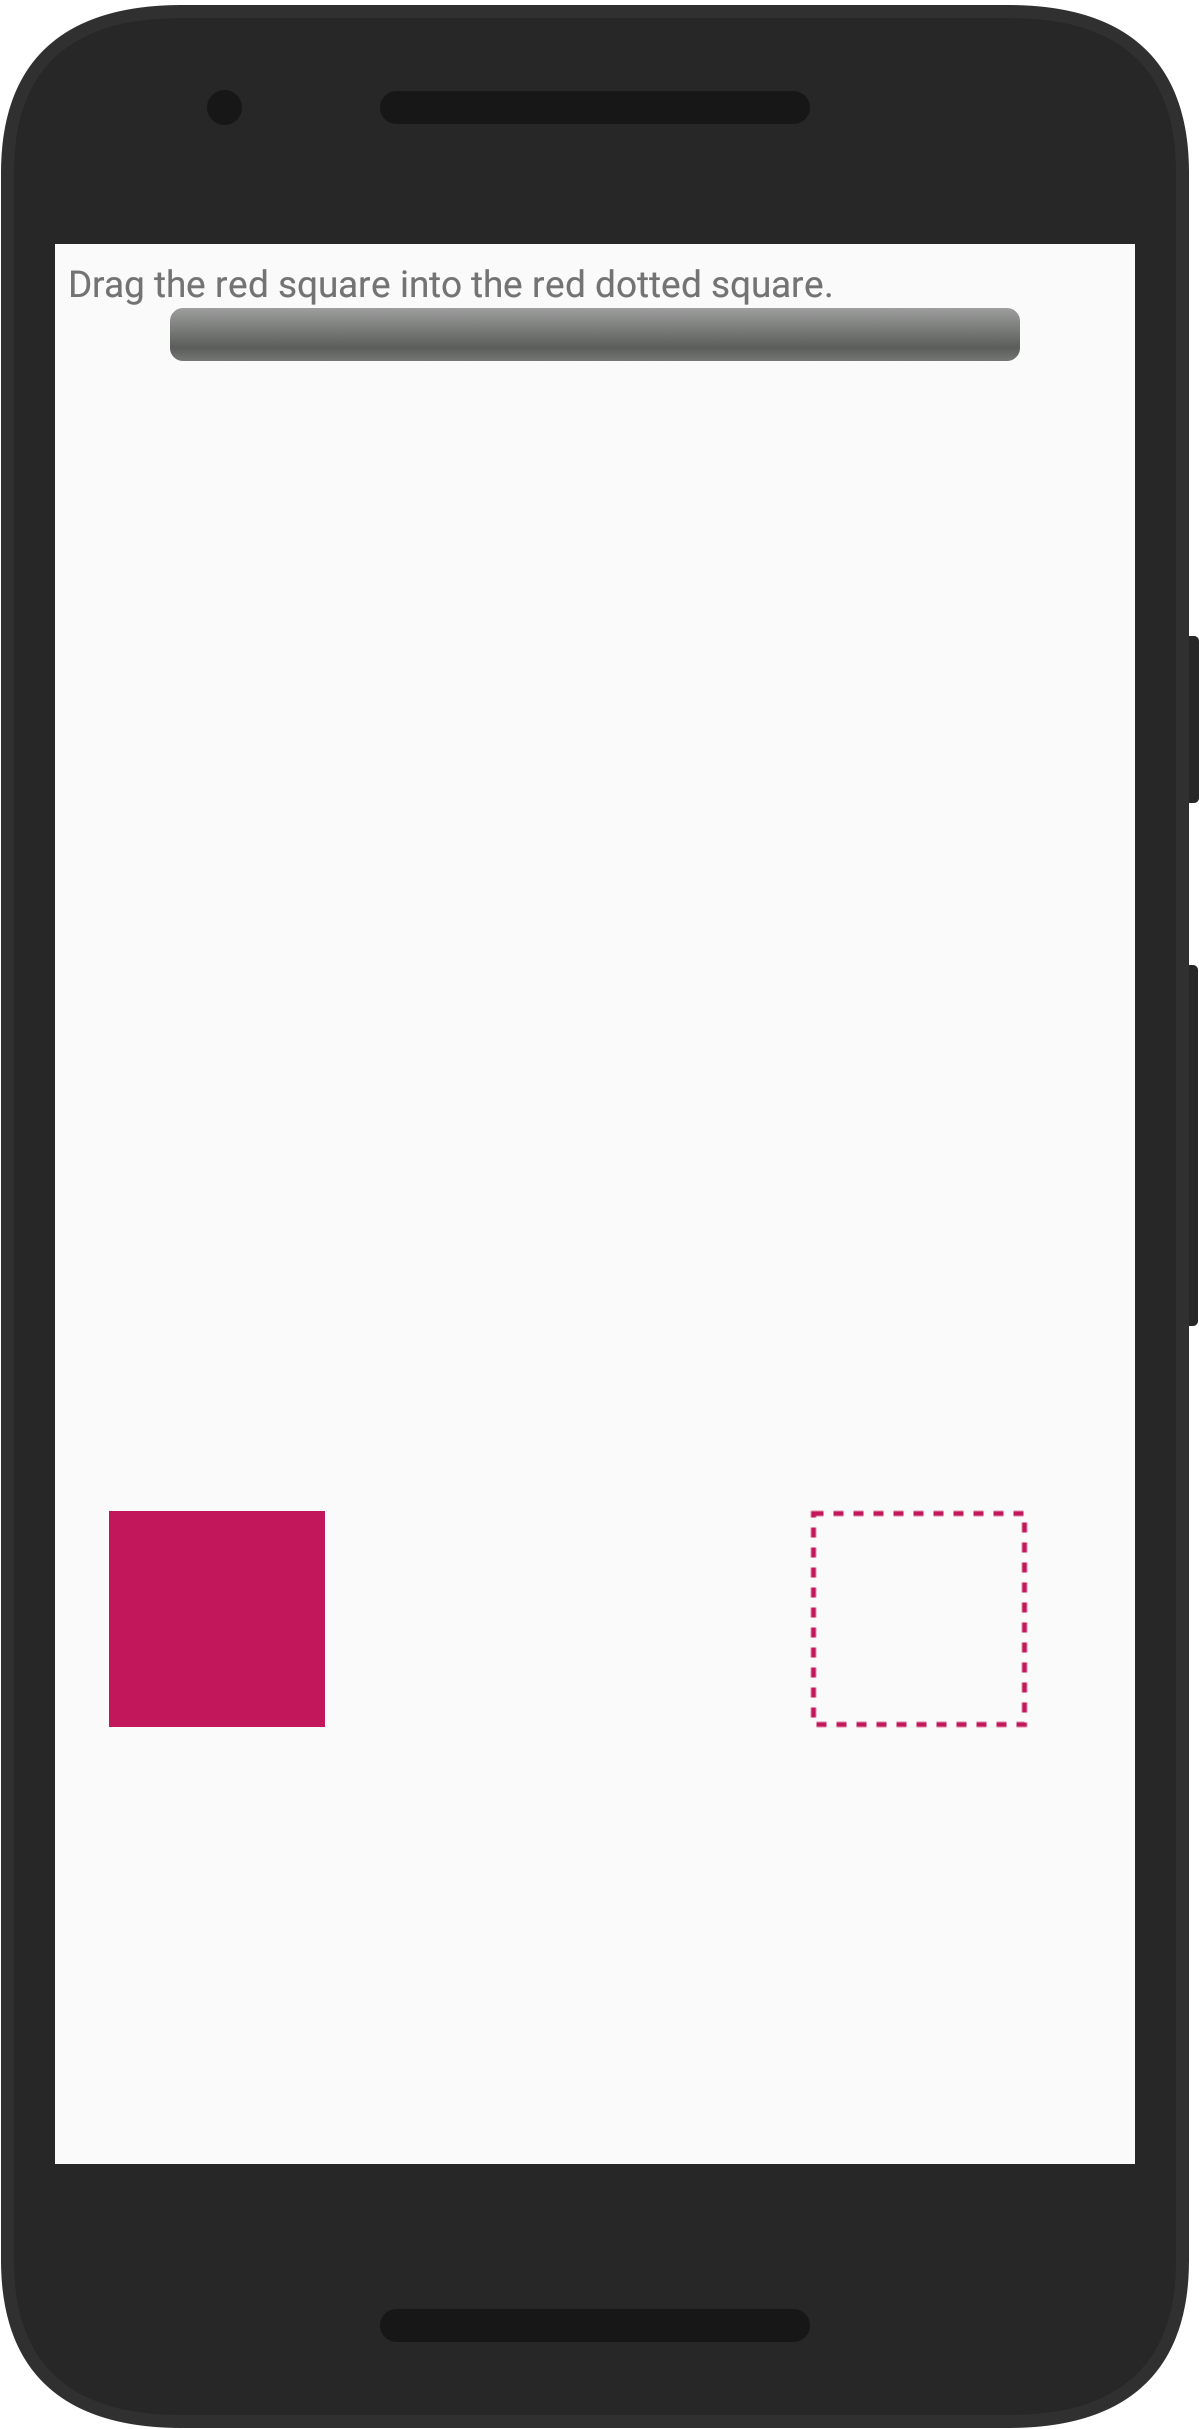
\includegraphics[height=\linewidth]{fitts}
	\caption{Fitts Law task with a progress bar displaying the current progress.}
	\label{fig:fittstask}
\end{marginfigure}

\section{Introduction}
Touch is the preferred input method on smartphones today. 
Current research and manufacturers are constantly trying to improve and enhance the interaction on smartphones. 
Enhancing smartphones with new, rich interaction methods allows users to operate their phone faster and more accurate, thereby increasing the usability and user-experience.
One way can be the extension of interactable space with interaction possibilities on the back of device (BoD) \cite{Le2016,Baudisch2009,Le2017}.
E.g. unlocking the phone by using gestures on the backside, or explicit touches on the backside to reach for unreachable targets on the front side may be possible applications of this technique.
However, some of these solutions do not conform with the form factors and weights of ordinary phones \cite{Corsten2017,DeLuca2013,Wolf2012}.
Another way to extend interaction is the introduction of additional touch gestures and touch recognition on touchscreens \cite{Le:2018:PalmTouch, Holz2015,Guo2015}.
Previous work tried predicting touch positions on the touchscreen based on sensor data from either built-in or additional sensors \cite{Le2017:Predic,MohdNoor2016}.\\
Accurately predicting touch positions could offer many use-cases:

\textbf{Preloading Content}: Preloading certain content that a user might request in the near future, e.g. a web page, reduces the waiting time and thus improves the user experience. 
	Removing the latency and thereby getting rid of the delay between certain actions greatly enhances the usability of a system. 
	However, when navigating on websites and preloading content from small links a high and precise accuracy is required. 
	Inaccurate prediction would require to preload more data around the predicted point.

\textbf{Highlighting Objects}: When navigating through folders, predicted future positions of a touch can be used to highlight information about the to be touched folders. 
	Navigation through a picture gallery on the phone can slightly enlarge the to be touched pictures to give a small preview, maybe showing picture information of where and when the picture was taken.
	The accuracy required for this approach does not necessarily have to be very high as elements are usually larger than small weblinks.

Despite its novelties, accuracy of some of these solutions has been low. In this paper, motivated by related work and its unexploredness, we present a machine learning model for predicting touches on smartphones using only the phones' built-in sensors.


\textbf{Likewise, traditional touch events fire at the moment one makes contact with the digitizer, yet the genesis of the grasping or aiming movement comes much earlier, and originates away from the screen itself. }

